\documentclass[a4paper,12pt]{report}
\usepackage{tkz-tab}
\begin{document}
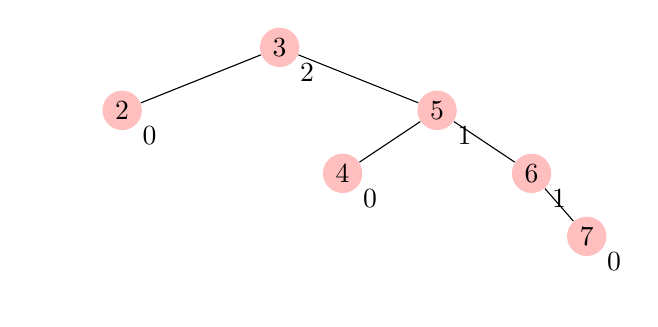
\begin{tikzpicture}[label distance =-1mm]
\tikzstyle{noeud}=[circle, minimum size=5mm, inner sep=0pt, fill=red!25!white]
\tikzstyle{level 1}=[sibling distance=40mm, level distance=8mm]
\tikzstyle{level 2}=[sibling distance=24mm, level distance=8mm]
\tikzstyle{level 3}=[sibling distance=14mm, level distance=8mm]
\tikzstyle{level 4}=[sibling distance=8mm, level distance=8mm]
\node[noeud,label=330:$2$] {3}
child
{node[noeud,label=330:$0$] {2}
child
{{edge from parent[draw=none]}}
child
{{edge from parent[draw=none]}}
}
child
{node[noeud,label=330:$1$] {5}
child
{node[noeud,label=330:$0$] {4}
child
{{edge from parent[draw=none]}}
child
{{edge from parent[draw=none]}}
}
child
{node[noeud,label=330:$1$] {6}
child
{{edge from parent[draw=none]}}
child
{node[noeud,label=330:$0$] {7}
child
{{edge from parent[draw=none]}}
child
{{edge from parent[draw=none]}}
}
}
}
;
\end{tikzpicture}

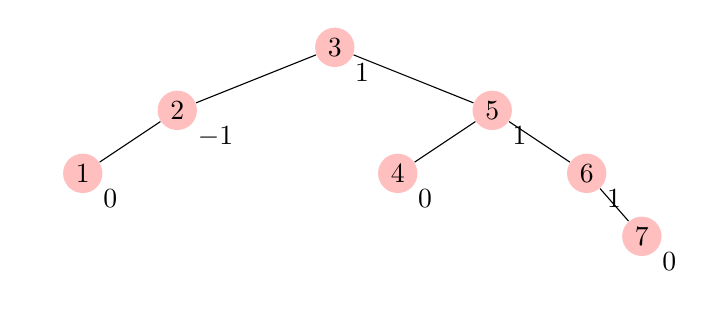
\begin{tikzpicture}[label distance =-1mm]
\tikzstyle{noeud}=[circle, minimum size=5mm, inner sep=0pt, fill=red!25!white]
\tikzstyle{level 1}=[sibling distance=40mm, level distance=8mm]
\tikzstyle{level 2}=[sibling distance=24mm, level distance=8mm]
\tikzstyle{level 3}=[sibling distance=14mm, level distance=8mm]
\tikzstyle{level 4}=[sibling distance=8mm, level distance=8mm]
\node[noeud,label=330:$1$] {3}
child
{node[noeud,label=330:$-1$] {2}
child
{node[noeud,label=330:$0$] {1}
child
{{edge from parent[draw=none]}}
child
{{edge from parent[draw=none]}}
}
child
{{edge from parent[draw=none]}}
}
child
{node[noeud,label=330:$1$] {5}
child
{node[noeud,label=330:$0$] {4}
child
{{edge from parent[draw=none]}}
child
{{edge from parent[draw=none]}}
}
child
{node[noeud,label=330:$1$] {6}
child
{{edge from parent[draw=none]}}
child
{node[noeud,label=330:$0$] {7}
child
{{edge from parent[draw=none]}}
child
{{edge from parent[draw=none]}}
}
}
}
;
\end{tikzpicture}

\end{document}
